%----------------------------------------------------------------------------------------
%	FOCAL PLANE RECONSTRUCTION
%----------------------------------------------------------------------------------------
%\section{Focal Plane Geometry}
%\label{se:geometry}

The FOV reconstruction consists in matching the KID frequency tones
to positions in the sky and in performing a KID selection. Although all
the (2,900) design KID are responsive, some of them are affected by
cross-talk or are noisy due to an inacurrate tuning of their
frequency, and must be discarded for further analysis. We use \bms,
which allow projecting an individual map per KID as discussed in
Sect.~\ref{se:beammaps}, to measure the KID positions and relative gains, as
discussed in Sect.~\ref{se:fov_geometry}. The measured KID positions
are further
checked by matching with the design positions, as presented in
Sect.~\ref{se:grid_distortion}. In Sect.~\ref{se:avg_kidpar}, we
present the final KID selection and FOV geometry, as obtained by
repeating the procedure on a series of \bms.  



%   Methods
%----------------------------------------------------------------------------------------
\subsection{Reconstruction of the FOV positions}
\label{se:fov_geometry}

In order to be able to produce a map, one needs to associate a pointing
direction to any data sample of the system. The telescope provides us with
various pointing information for a reference position in the focal plane. We
then need to know the relative pointing offsets of each detector. We use
\bms\ for this purpose (see Sect.~\ref{se:beammaps}). The determination of the
KID offsets in the focal plane proceeds in two steps.

\paragraph{Step 1.} We apply a median filter per
KID timeline whose width is set to 31 samples, that is equivalent to
about 5~FWHM at 65 arcsec/s and for the sampling frequency of
23.84~Hz. Then, we project one map per KID in Nasmyth
coordinates. The median filter removes
efficiently most of the low frequency atmospheric and electronic
noise, albeit with a slight ringing and flux loss on the
source. However, at this stage, we are only interested in the location
of the observed planet.
To derive the Nasmyth coordinates from the
provided $(\alpha_t,\delta_t)$ and $(\Delta\alpha_t,\Delta\delta_t)$
coordinates, we build the following quantities at time~$t$:

\begin{eqnarray}
\Delta x_t &=& \cos\delta_t \Delta\alpha_t - \sin \delta_t\Delta \delta_t \nonumber \\
\Delta y_t &=& \sin\delta_t \Delta\alpha_t + \cos \delta_t\Delta \delta_t \nonumber
\end{eqnarray}

Note that $\Delta\alpha_t$ is already corrected by the $\cos\delta_t$ factor to
have orthonormal coordinates in the tangent plane of the sky and be immune to
the geodesic convergence at the poles. Moreover, before projecting the
time-ordered data onto maps, we check
the accuracy of the time-stamping and the consistency between the
telescope time and NIKA2 time. First, we test the
synchronisation of the electronic boxes and the regularity of the
time increase. In case of detection of an anomaly, the
time-stamping of the impacted data samples is
recalculated by interpolating from the accurately stamped
neighbour samples. Then, a so-called \emph{zigzag}
procedure is used to test for delay between the telescope pointing
information and NIKA2 timelines: we fit a constant shift between the
source positions estimated using the subscans in one direction and
using the subscans in the opposite direction. The data timelines are
then projected onto maps. 
We fit a 2D elliptical Gaussian on
each KID map. The centroid of this Gaussian is a first estimate of the KID
offsets, FWHM, ellipticity and sensitivity. We apply a first KID selection by
removing outliers to the statistics on these parameters. We also discard
manually KIDs that show a cross-talk counterpart on their map.

\paragraph{Step 2.} With these offsets, it is already possible to
produce maps from the combination of all detectors. However, for
accurate calibration, we must correct for the flux loss
induced by the median filter and ensure that each timeline is treated
in the same way as the final observation will. For this, we apply the
pointing reconstruction and the noise subtraction presented in
Sect.~\ref{se:dataproc}.
At this stage, we do not have
absolute calibration for each KID (no opacity correction yet) but the
amplitude of the fitted centroid on the same planet provides the required
cross-calibration between KIDs. The final absolute calibration will be
presented in Sect.~\ref{se:calibration}.\\

This analysis is repeated on all \bms\ to obtain statistics and
precision on each KID parameter, together with estimates on KID
performance stability, as discussed in the next sections.

\begin{figure*}[!thbp]
\begin{center}
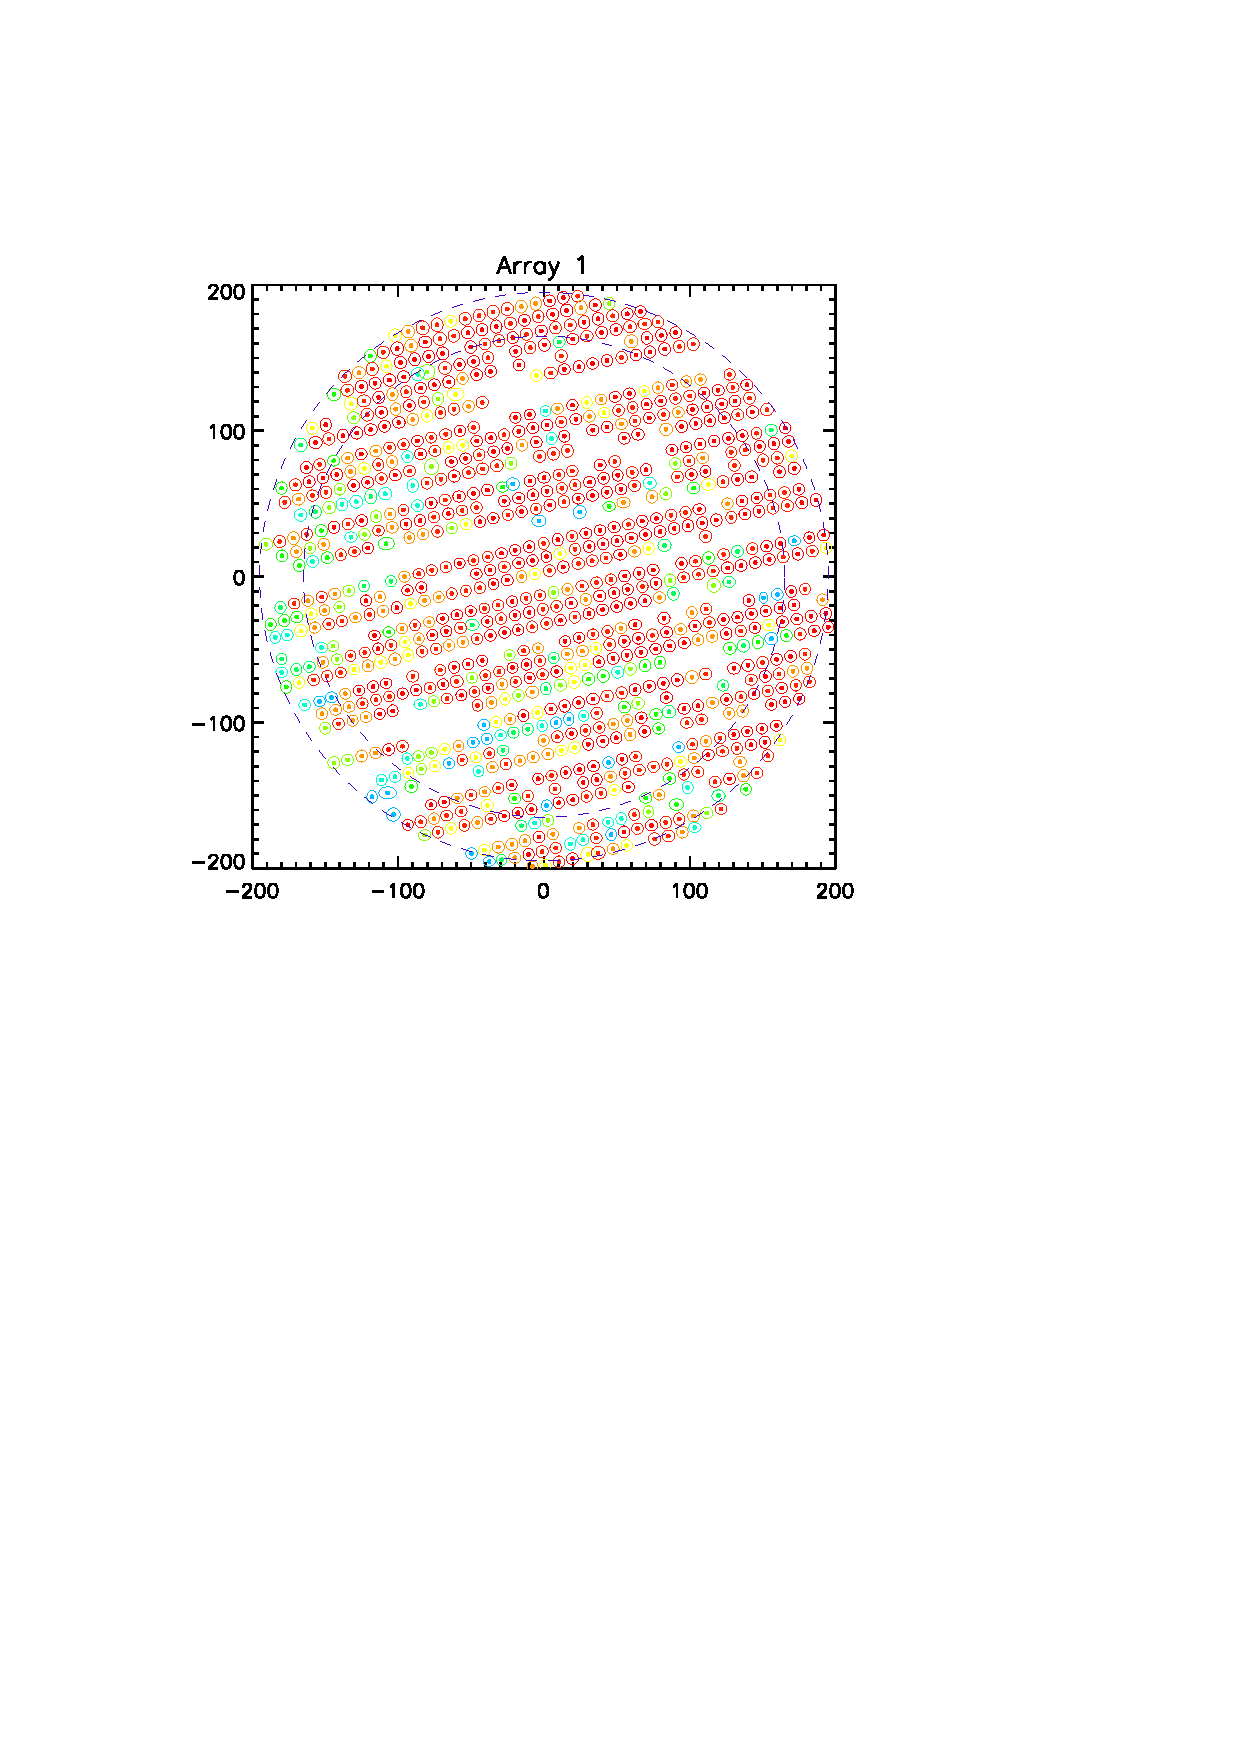
\includegraphics[trim=3cm 14cm 6cm 4cm, clip=true, width=0.32\linewidth]{Figures/A1_fwhm_color_count.pdf}
%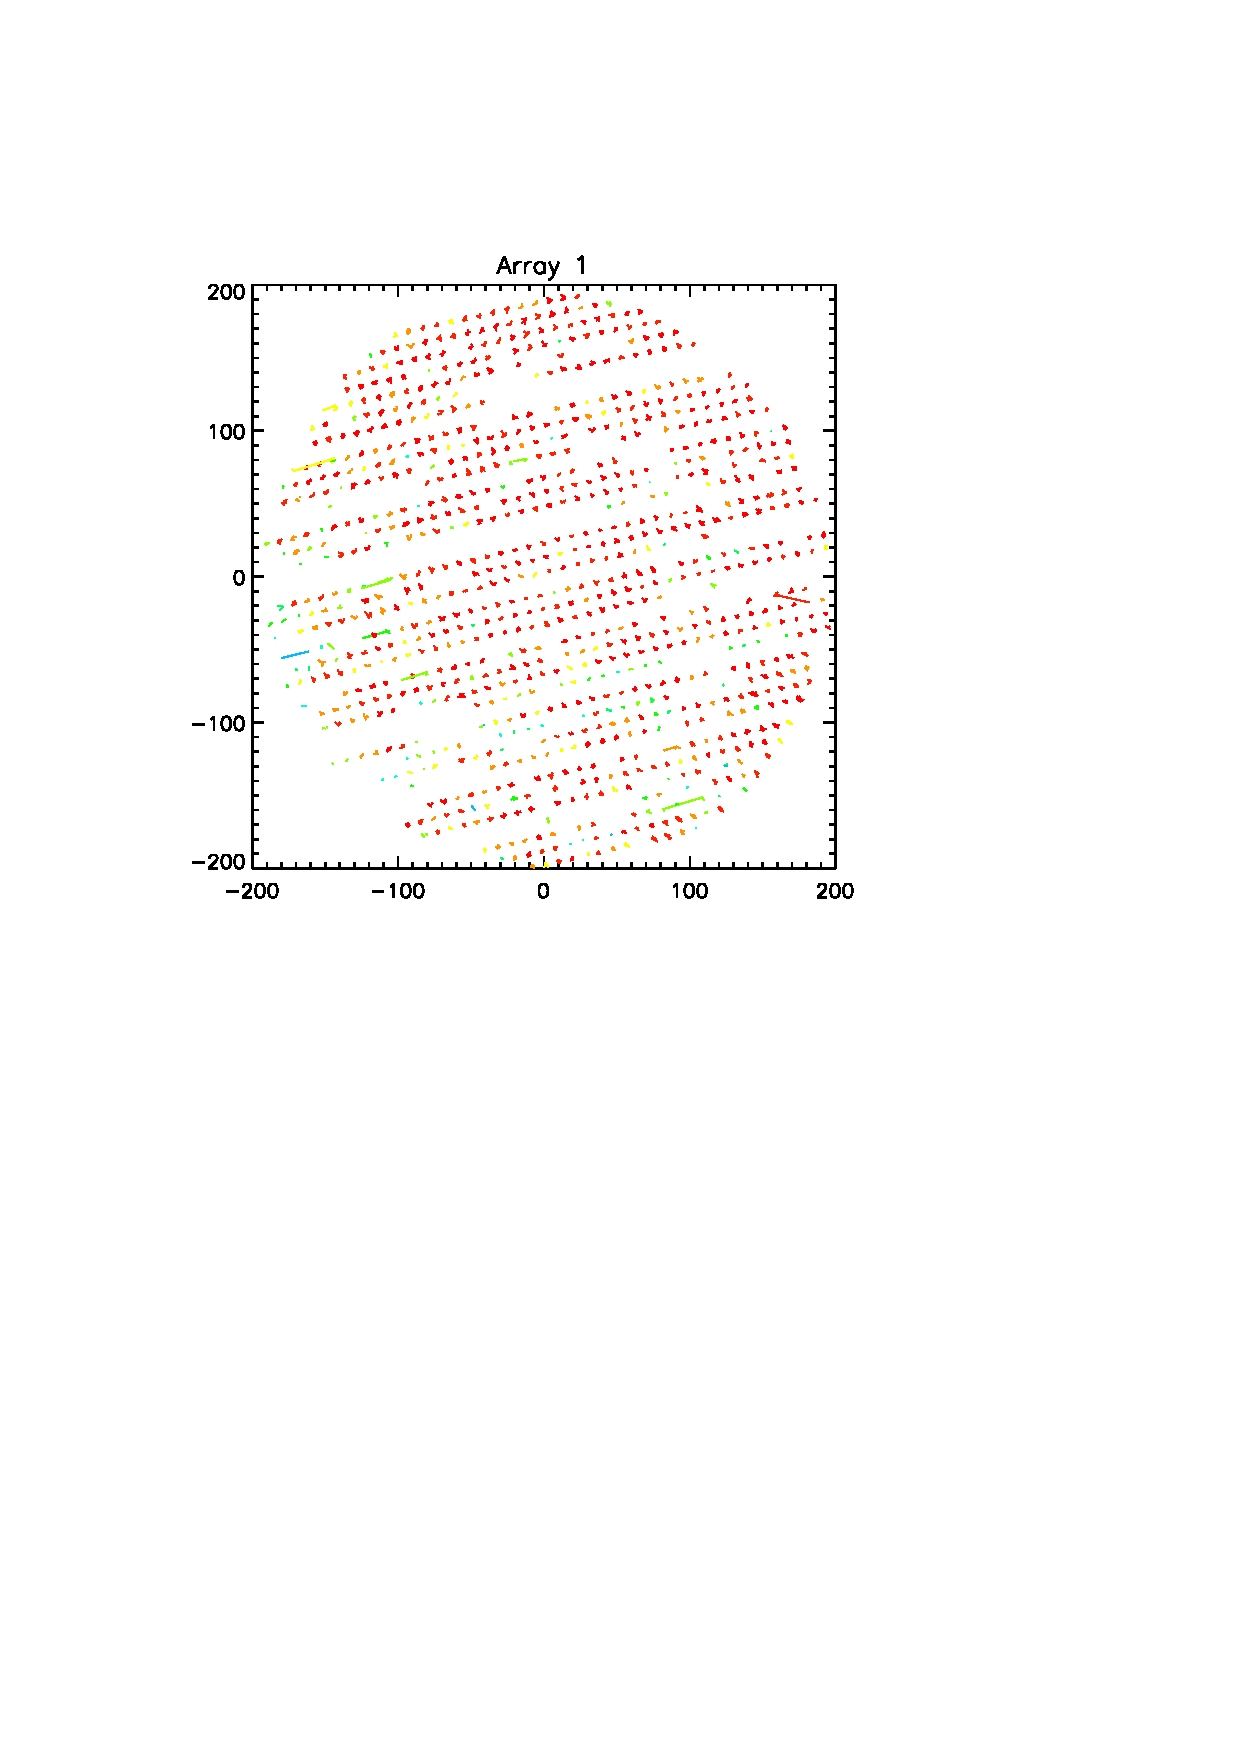
\includegraphics[trim=2cm 14cm 5cm 4cm, clip=true,width=0.45\linewidth]{Figures/A1_positions.pdf}
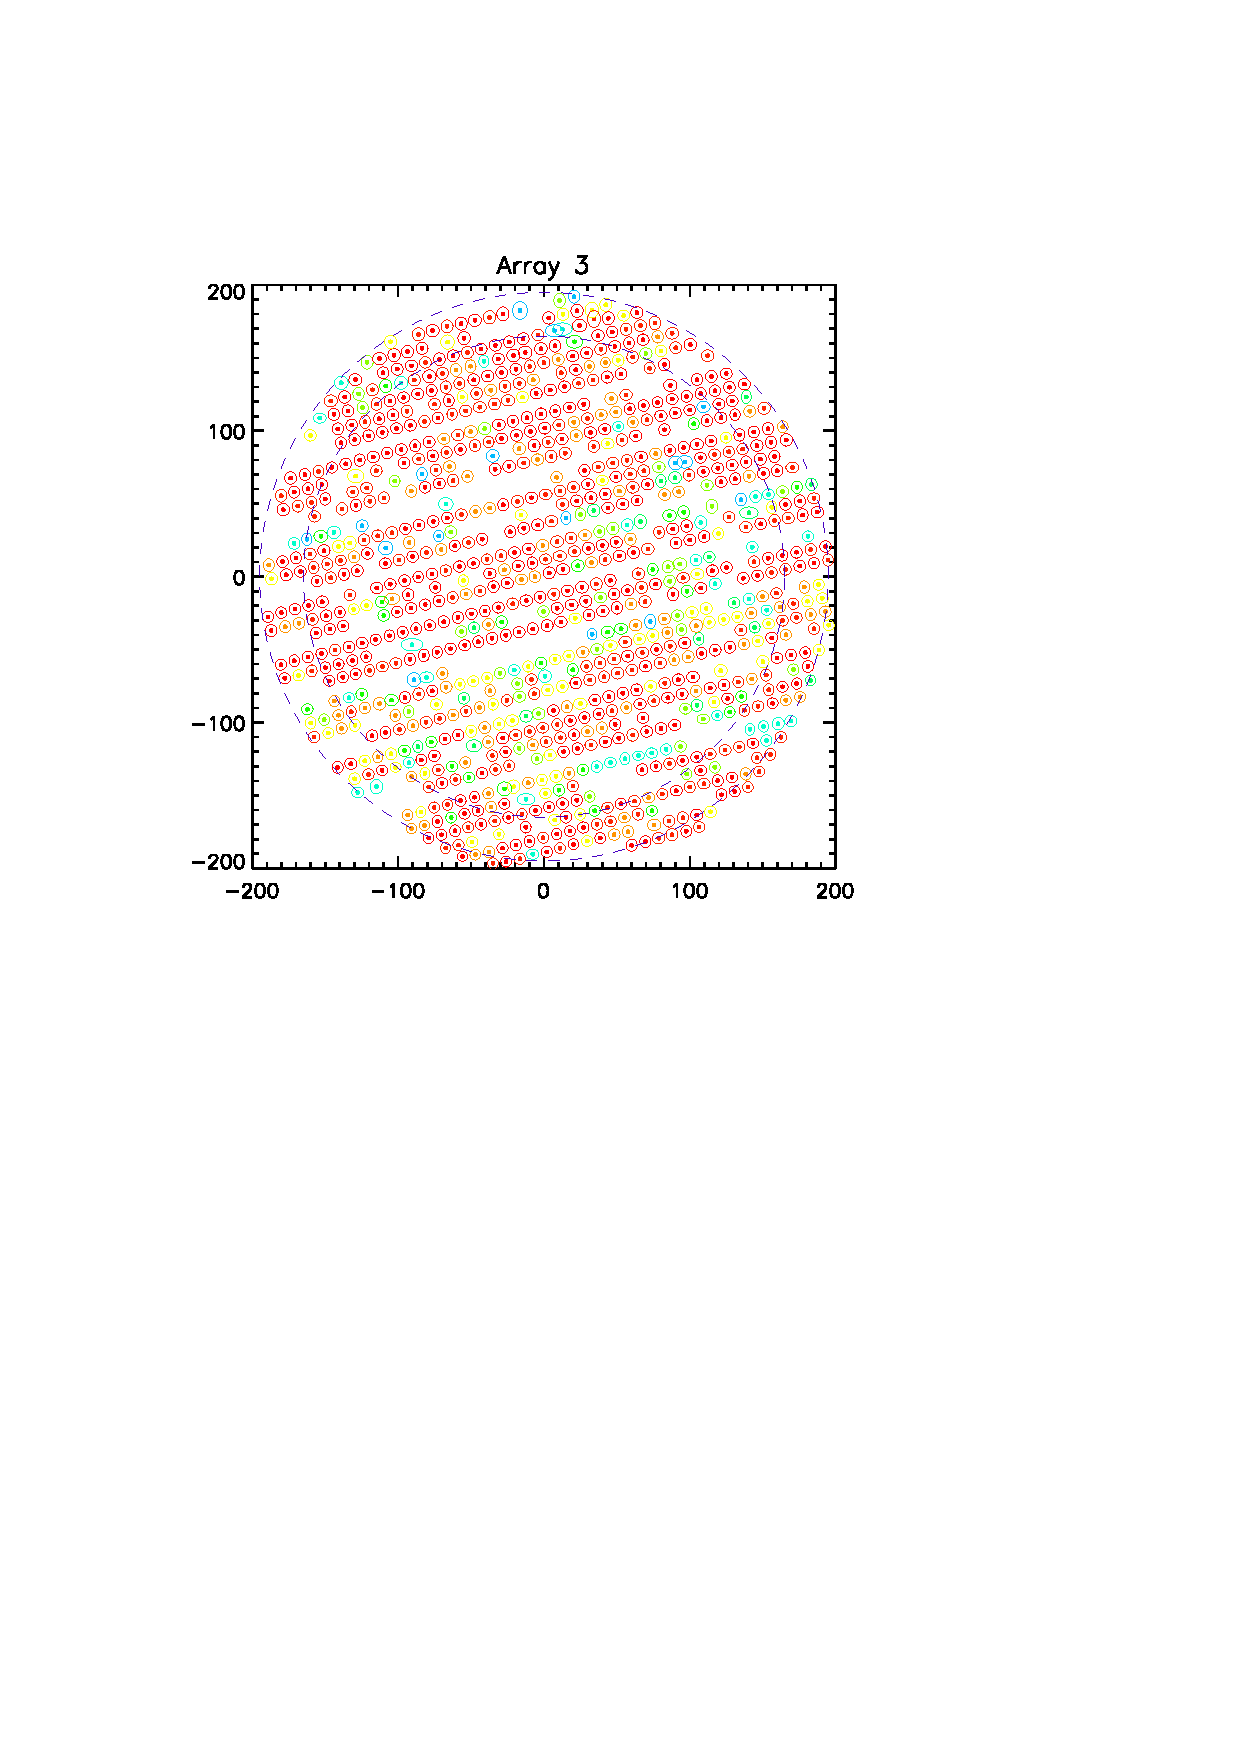
\includegraphics[trim=3cm 14cm 6cm 4cm, clip=true, width=0.32\linewidth]{Figures/A3_fwhm_color_count.pdf}
%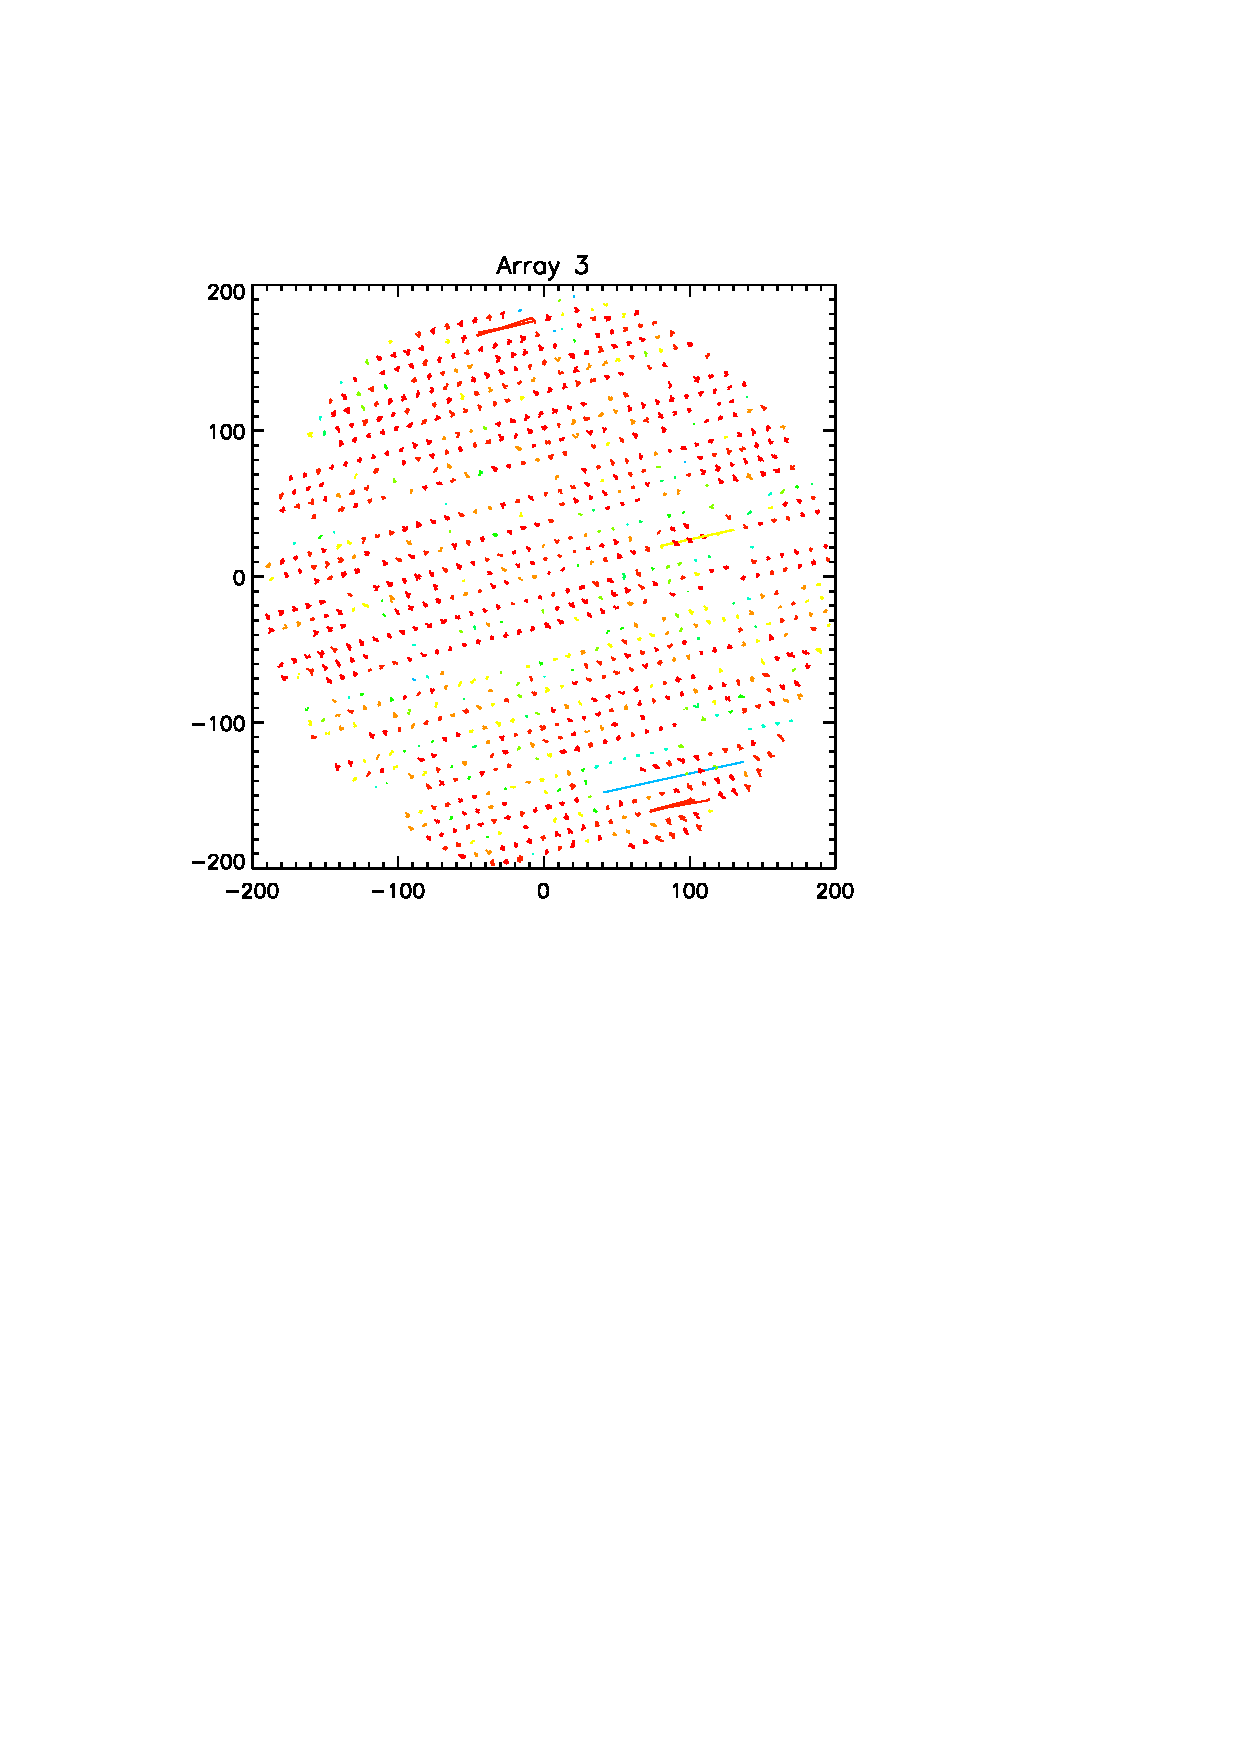
\includegraphics[trim=2cm 14cm 5cm 4cm, clip=true,width=0.45\linewidth]{Figures/A3_positions.pdf}
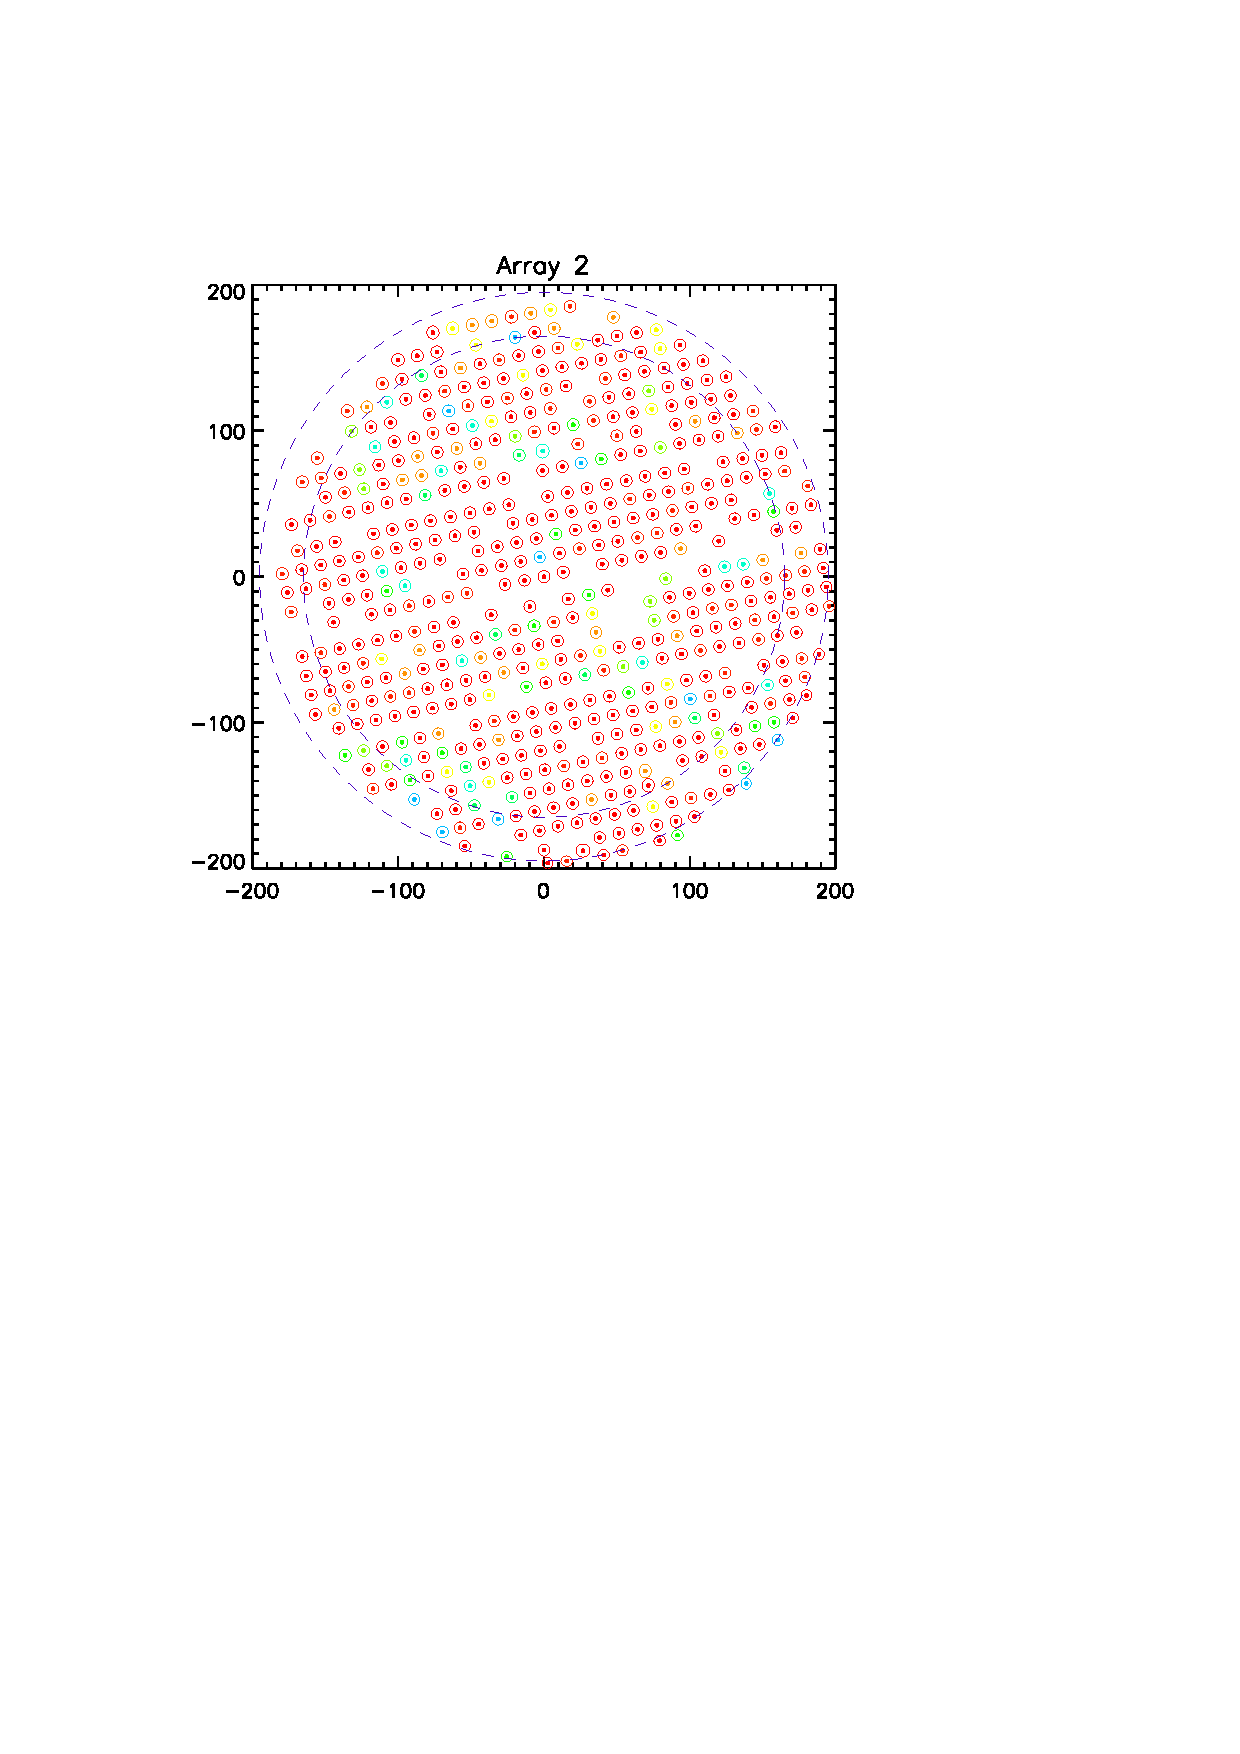
\includegraphics[trim=3cm 14cm 6cm 4cm, clip=true, width=0.32\linewidth]{Figures/A2_fwhm_color_count.pdf}
%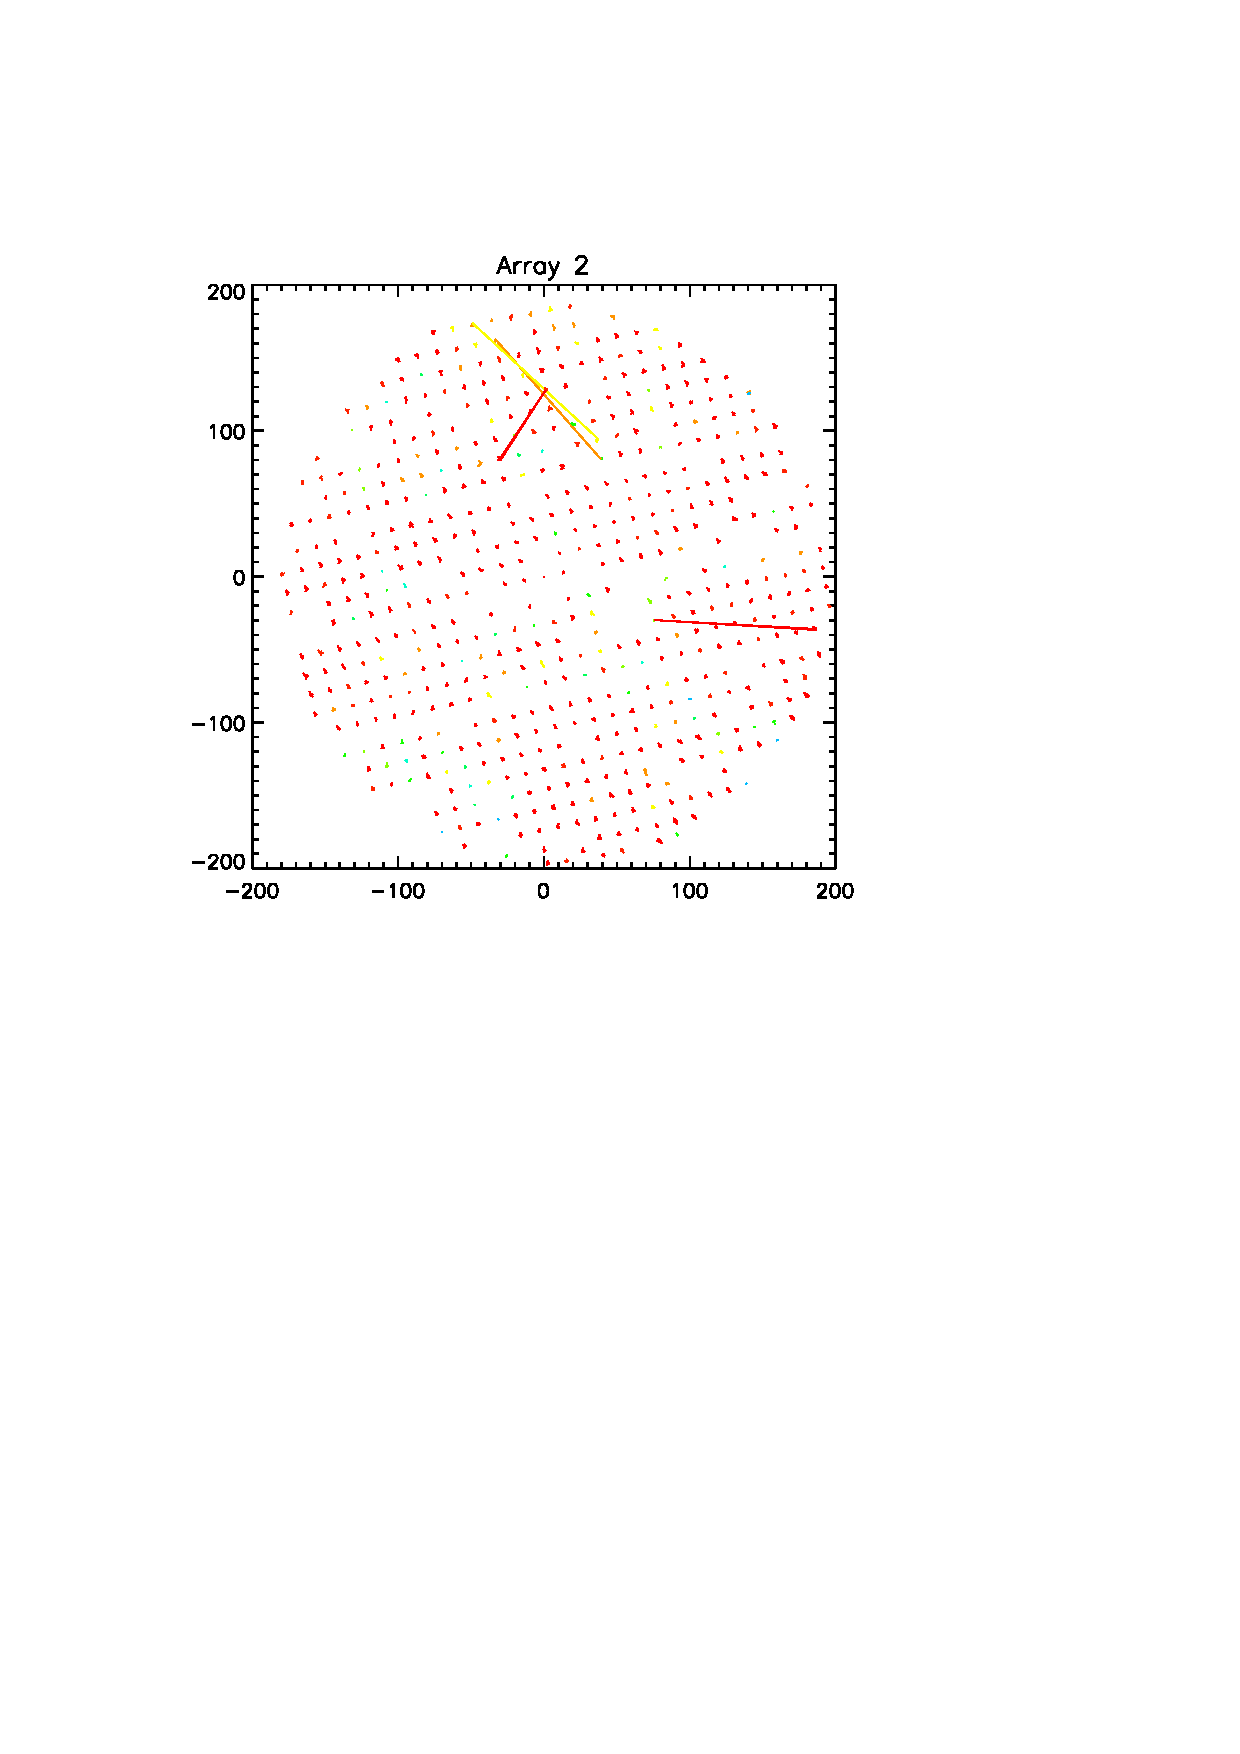
\includegraphics[trim=2cm 14cm 5cm 4cm, clip=true,width=0.45\linewidth]{Figures/A2_positions.pdf}
\caption[KID selection in the FOV]{Average detector positions
  for arrays A1, A3, and A2. The three plots show the detectors that
  met the quality criteria for at least two \bms\ during two technical
  campaigns: 952, 961, and 553 for A1, A3 and A2, respectively. The color
  indicates, from green to red, how many times a KID was
  identified as valid on a \bm. The inner and outer
  dash-line circles correspond to a FOV of 5.5\,arcmin and 6.5\,arcmin,
  respectively. Units are arcseconds.}
\label{fig:avg_fov_color}
\end{center}
\end{figure*}

\subsection{FOV grid distortion}
\label{se:grid_distortion}

We compare the reconstructed KID position in the FOV to their design
position in the array. We fit the field translation and rotation that allow
matching the measured KID positions with the design positions using a 2D
polynomial mapping function of degree one. We call distortion cross-terms
between the two spatial coordinates in the polynomial fit.

The aim is twofold. First we obtain a detailed
characterisation of the real geometry of NIKA2 focal plane. Secondly,
this analysis constitutes the last step of the KID
selection, and the most deviant KIDs, whose measured position is found
above $4''$ from the design position are discarded. 


We present the global results of the grid distortion
analysis using the KID positions given
by the focal plane geometry procedure, as described in
Sect.~\ref{se:fov_geometry}, applied to three \bm\ scans acquired
during the N2R9 campaign. Note that the selected KID numbers are low
in this example as the scans were acquired during the daytime
and suffers from temperature-induced instabilities (see
Sect.~\ref{se:beam_variation}).
The results are gathered in Table~\ref{ta:gridmatch}.

\begin{table}[!htbp]
  \caption[Field-of-view deformations]{Linear 2D fit of the observed
    position of the detectors in the sky for the N2R9 campaign against
    their mechanically
    designed position. The initial table of selected KIDs is given
    by the focal plane geometry procedure, as described in
    Sect.~\ref{se:fov_geometry}, applied to three \bm\ scans acquired
    during N2R9. Note that the selected KID numbers are particularly
    low in this example, as the scans were observed during the daytime
    and suffer from temperature-induced instabilities (see
    Sect.~\ref{se:beam_variation}). Even in this pessimistic case,
    more than 90\% of the detectors are within less than 5 arcseconds
    of their expected position.}
  \label{ta:gridmatch}
  \centering
  \begin{tabular}{r|c|c|c}
    \hline
    \hline
    Characteristic &  Array 1  &	Array 3   &	Array 2  \\
    \hline
    \small{$\lambda$ [mm]}  &1.25     &      1.25      &    2.05   \\
    %&1140 	 &      1140 	  &    616       & \small{Total of designed KIDs (TDK)} \\
    \small{Selected KID}\tablefootmark{a}       &  736   & 758   & 444  \\
    \small{Well-placed KID}                  &  673   & 734   & 437  \\
    \small{Ratio [\%]}                       &  91   & 96   & 98  \\
    %&673/736  &	734/758   &    437/444   & \small{Well-placed KIDs (WPK)/Found KIDs (FK)} \\
    %&91/59 	 &      96/64 	  &    98/71 	 & \small{Ratio [\%] of WPK/FK and WPK/TDK} \\
    \small{Median deviation\tablefootmark{b}  [arcsec]}    &   0.87 	 &      0.84 	  &    0.66  \\
    \small{Mean distortion [arcsec]}                       &   0.52 	 &      0.69 	  &    0.68  \\
    \small{Array center\tablefootmark{c} [arcsec]}  & (2.3,4.5) &	(2.0,5.8)  &   (9.3, 7.5)  \\
    \small{Plate scaling\tablefootmark{d} [arcsec/mm]}   &  4.90     &	4.88      &    4.88 \\
    %& \small{Plate scaling [arcsec/mm] in the Design x and y (averaged)} \\
    \small{Plate rotation angle\tablefootmark{e} [degree]} & 77.3     &	76.4      &    78.2  \\
    %\small{FOV [arcmin] (Total KIDs)}                      & 6.6      &	6.6       &    6.6   \\
    \small{Grid step\tablefootmark{f} [arcsec, mm] }   & 9.8, 2.00 &	9.7, 2.00  &    13.3, 2.75 \\
    % Old values, rechecked (difference comes from lambda and D)
    %   1.24  &	1.22  &	0.97  &	Distance between near detectors with $30\,\rm{m}$ diameter aperture [in $\lambda$/D] \\
    % here new values checked FXD 30 Nov 2018:
    \small{Measured grid step[$\lambda$/D] } & 1.11     &	1.10      &	0.87  \\
    %\new{with $27\,\rm{m}$ effective diameter aperture} [in $\lambda$/D]} \\
    \small{Modeled grid step\tablefootmark{g} [$\lambda$/D]}  & 1.09     &      1.09      & 0.93    \\
    \hline
  \end{tabular}
  \tablefoot{ \\
    \tablefoottext{a}{Initial number of KIDs given in a FOV geometry
      for the N2R9 campaign (pessimistic case)}
    \tablefoottext{b}{Median deviation [arcsec] for detectors deviating by less than 5~arcsec}
    \tablefoottext{c}{Array center in Nasmyth coordinates}
    \tablefoottext{d}{Averaged scaling between the measured grid and the design grid}
    \tablefoottext{e}{Plate rotation from the design to Nasmyth coordinates}
    \tablefoottext{f}{Distance between neighbour detectors}
    \tablefoottext{g}{Distance between neighbour detectors modeled using ZEMAX simulation}
  }
\end{table}

It shows that on average the position of each detector is known to better than
an arcsecond. The 1\,mm arrays have almost the same center but this center
differs by 7 and 2\,arcsec in Nasmyth coordinates from the
2\,mm array center. The sampling is above
$\lambda/D$ at 1\,mm, assuming a 27\,m effective diameter aperture. Note that
the plate rotation angle was designed as 76.2\,degrees, less than 2
degrees from what is observed. We find that array 1
has some of the most deviant detectors (above 4\,arcsec from their expected
position). These detectors should be excluded from further analysis.

This has been compared to expectations obtained using ZEMAX
simulation. 
%The grid diagram generated using ZEMAX provides us with
%the maximum dispersion in the field defined by
%
%\begin{equation}
%P = \frac{\sqrt{(x_p - x_r)^2 + (y_p - y_r)^2}}{\sqrt{x_p^2 + y_p^2}},
%\end{equation}
%
%where $(x_p, y_p)$ and $(x_r, y_r)$ are respectivelly the predicted
%and real coordinates on the image surface relative to the reference
%field position image location (see page 170 of the ZEMAX manual, 2007).
%The predicted coordinates for the whole field are obtained using a
%linear interpolation of a small area in the field central part,
%whereas the real coordinates are calculated by ray tracing through the
%optical system.
%
%\begin{figure}[ht] 
%\begin{center}
%  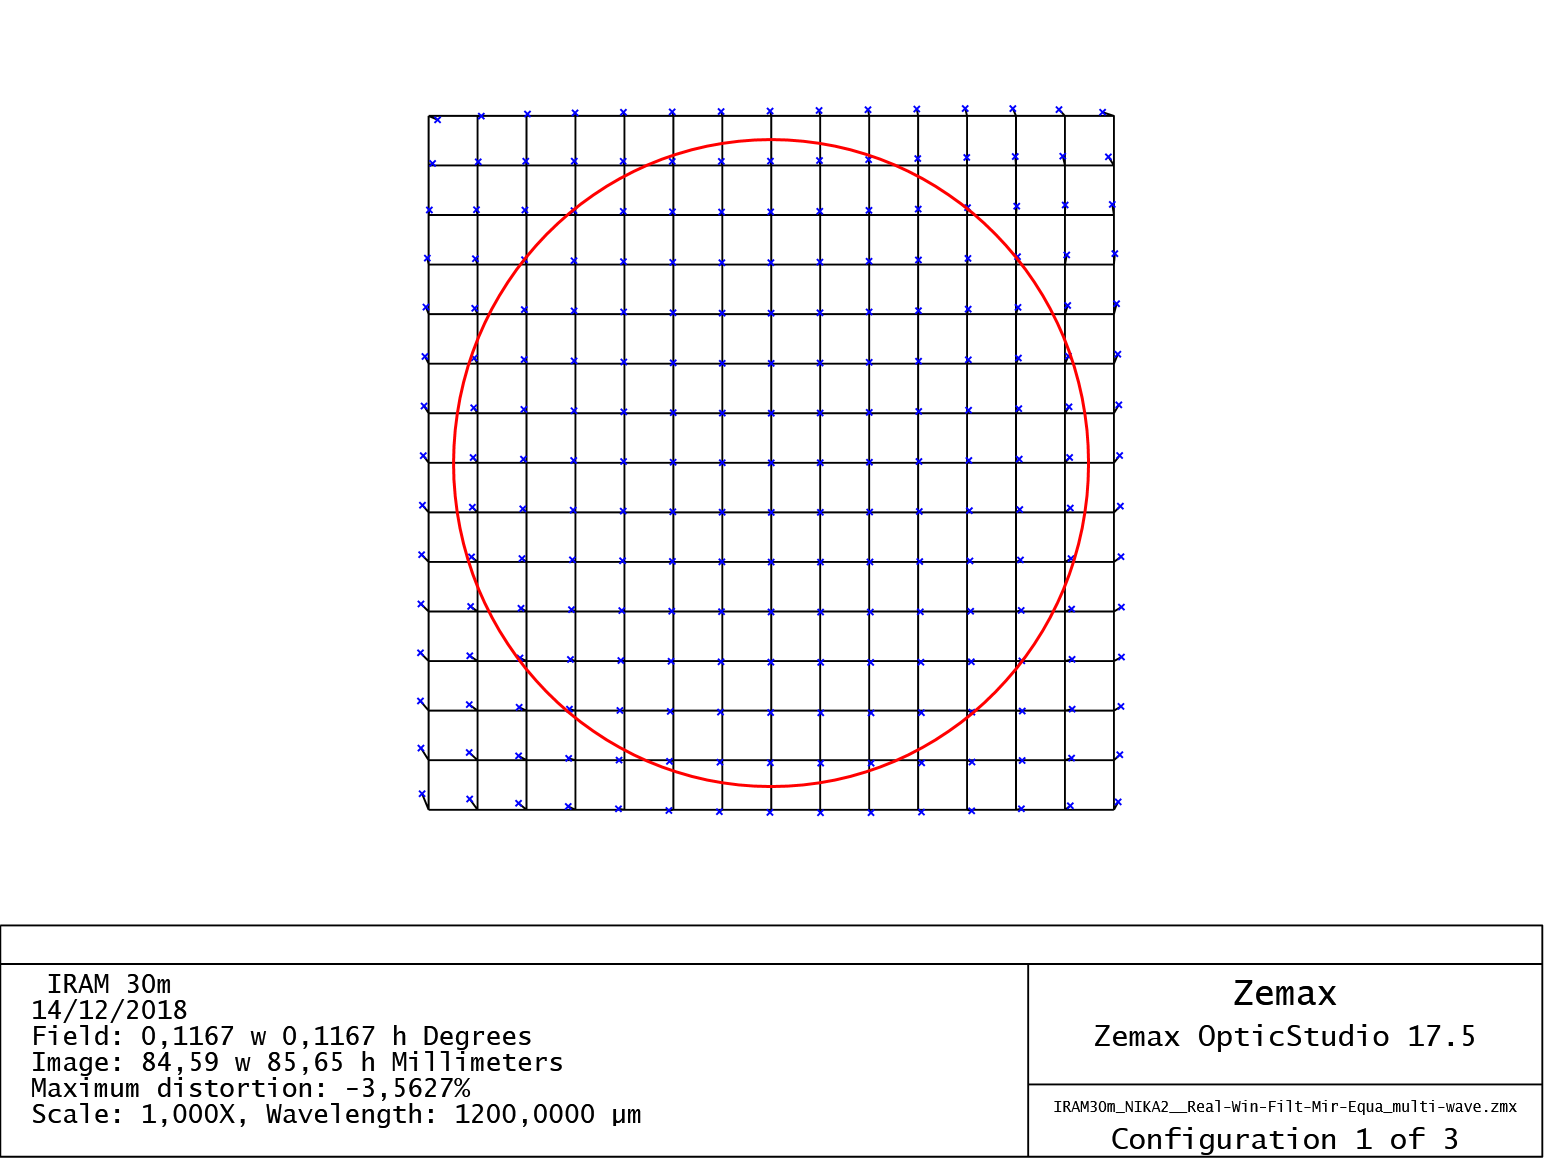
\includegraphics[width=0.9\textwidth]{Figures/NIKA2_Grid-distortion.png}
%  \caption[Simulated FOV grid]{NIKA2 grid diagram simulated using
%    ZEMAX. \new{The step of the grid is of 30 arcsec and the side width
%      of the black square is of seven arcmin. The red circle corresponds to the 
%      $6.5\,\rm{arcmin}$ diameter FOV. Blue crosses show the grid
%      distorsions in az-el coordinates and in the case of an observing
%      elevation of $14^o$. These grid distorsions depends on the
%      telescope elevation, whereas in the image plane (the plane of the
%      KID arrays) the distorsions are invariant. This allows for
%      concluding that the grid distorsions are caused by the optical
%      elements located between M4 and the dichroic plate.} 
%  }
% \label{fig:fov_grid_distortion_zemax}
%\end{center}
%\end{figure}
%Figure \ref{fig:fov_grid_distortion_zemax} shows the ZEMAX grid diagram for
%NIKA2 simulated optic system.
%
We generated a grid diagram for NIKA2 optic system and found a maximum
grid distortion of $2.7\%$ in the $6.5'$ FOV. We notice that the
strongest distortion appear in the upper right corner of the Nasmyth plan, which is
also the area of the largest defocus w.r.t. to the center (see
Sect.~\ref{sec:focus_surfaces}).
An expected distortion of $2.7\%$ is at most a 5'' shift from the
center to the outside of the array. The quoted distortions between the
measured and designed positions are thus consistent with the expected
maximum distortions from the NIKA2 optics.

%Auxillary information on this work can be found in this wiki post\footnote{\tiny
%  {\tt http$://$www.iram.fr$/$wiki$/$nika2$/$index.php$/$April$\_$19,$\_$2017,$\_$FXD,$\_$KID$\_$position$\_$mapping$\_$and$\_$Field$\_$distortion$\_$for$\_$Run9}}.
% FXD: this would need to be more ascertained. Lack of time to go further.


\subsection{KID selection and average geometry}
\label{se:avg_kidpar}

In order to identify the most stable KIDs, we compare the KID parameters
obtained with several \bms.  In the following, we show results as obtained using
seven \bms\ acquired during two technical observation campaigns in
2017.
%from Run10, two from Run9 and one from Run8.
For each KID we
compute the average position on the focal plane and the average FWHM, counting
the times that it has been considered as valid and at the same position. Indeed,
a few KIDs have close resonances and can be tuned and switched on some scans. A
few others must also be discarded because they appear identical numerically due
to the fact that a same (noisy) KID can sometimes be associated
to two different frequency tone in the acquisition.
These KIDs are flagged out (less than 1\% of the designed KIDs).

In Fig.~\ref{fig:avg_fov_color} we show the
average focal plane reconstruction, from green to red depending on the number of
times that the KID has been considered as valid.
The eight internal readout feed lines that connect each of the two
$1\,\rm{mm}$ arrays are also noticeable in this figure: first, slightly
larger spaces are seen between KID rows connected to different
feed-lines than between KID rows of the same feed line and second, KIDs at the end of a
feed line are less often valid than others (see e.g. the FOV of
Array 3). For A1, this end-of-feedline effect is mixed with the
effect of the KID gain variation across the FOV, which mainly affects
the South-West third of the array, as discussed in Sect.~\ref{se:flat_field}.

For A1, A3 and A2, respectively, we have 952, 961, and 553 KIDs that
have been considered as valid at least twice (840, 508, 868 valid at
least five times). Using this criterion, we deduce the fraction of
valid detectors over the designed ones, as given in Table~\ref{tab:number_of_kids}.

%% \begin{figure}[htp]
%% \begin{center}
%% 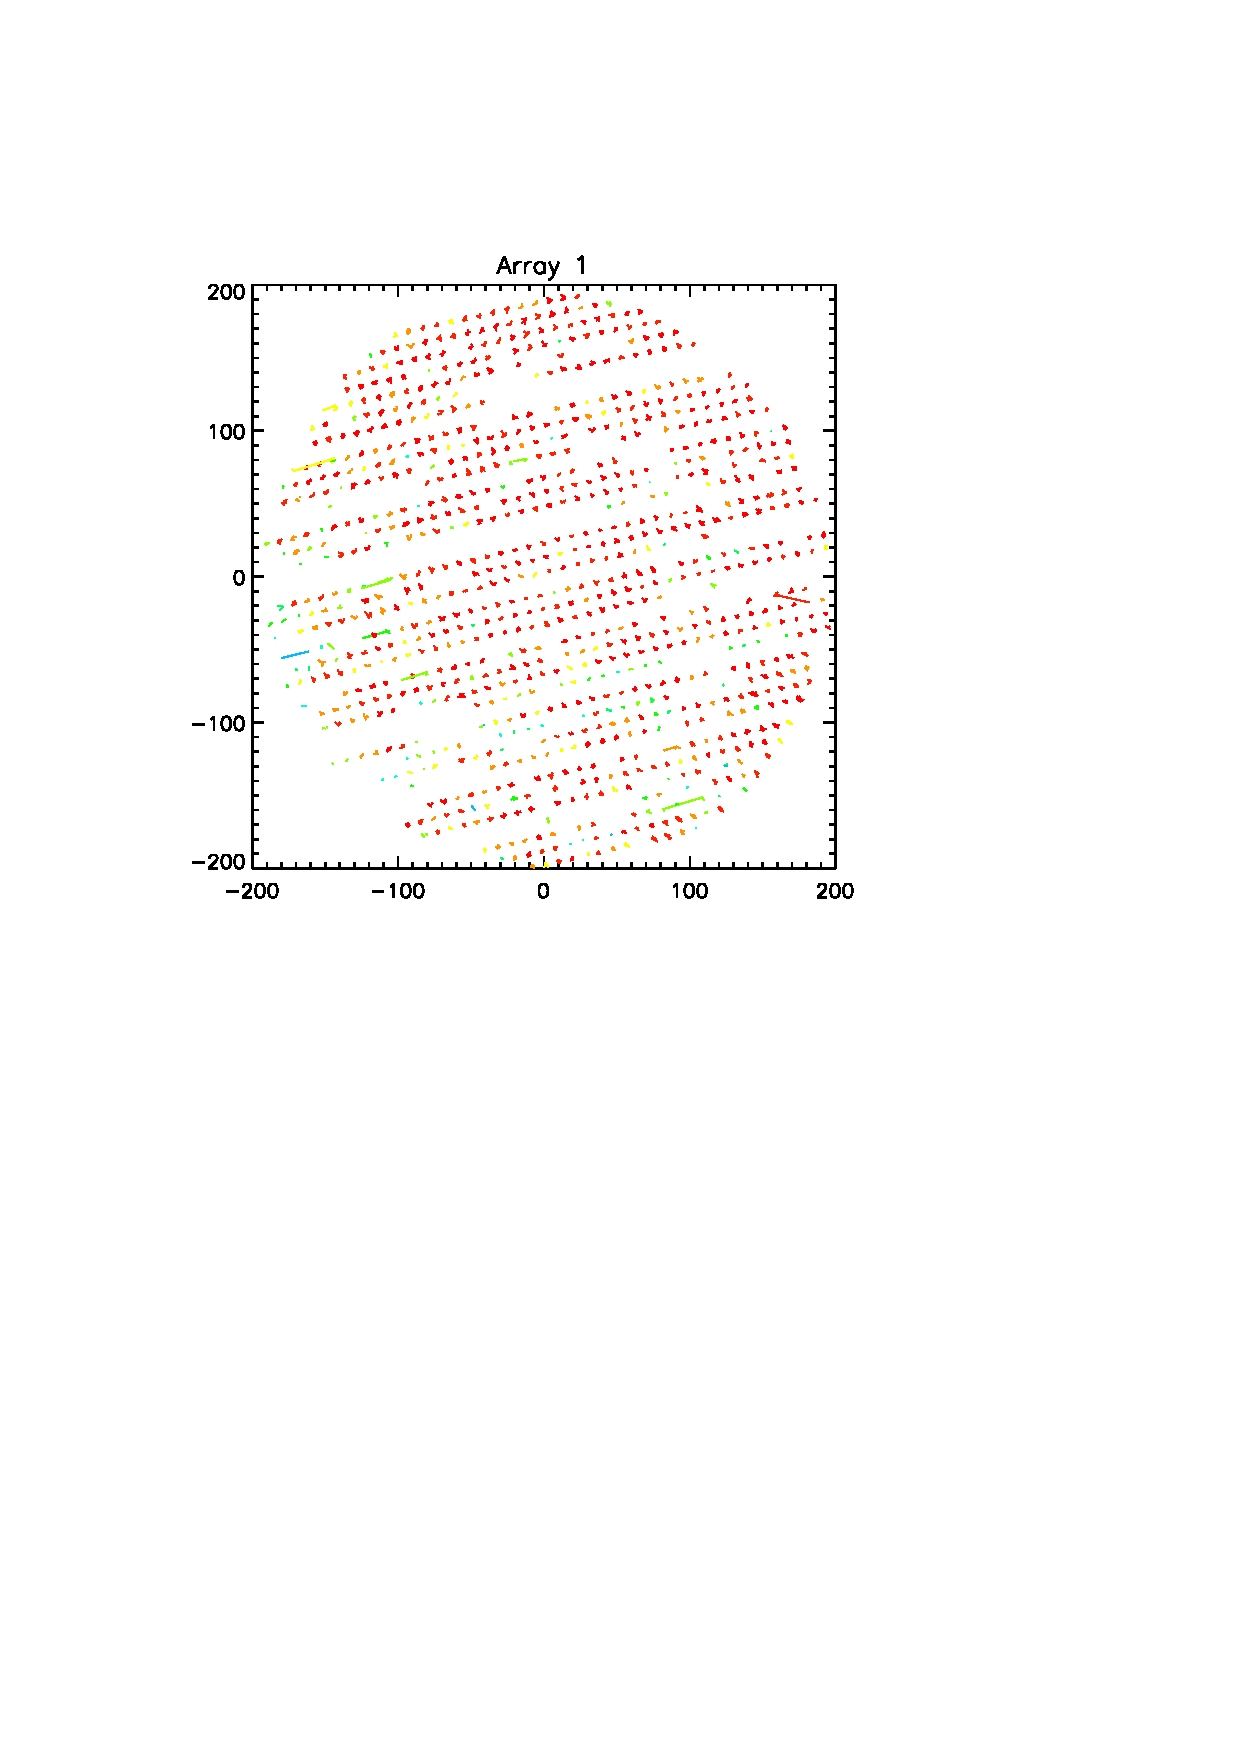
\includegraphics[trim=2cm 14cm 5cm 4cm, clip=true,width=0.55\linewidth]{Figures/A1_positions.pdf}
%% 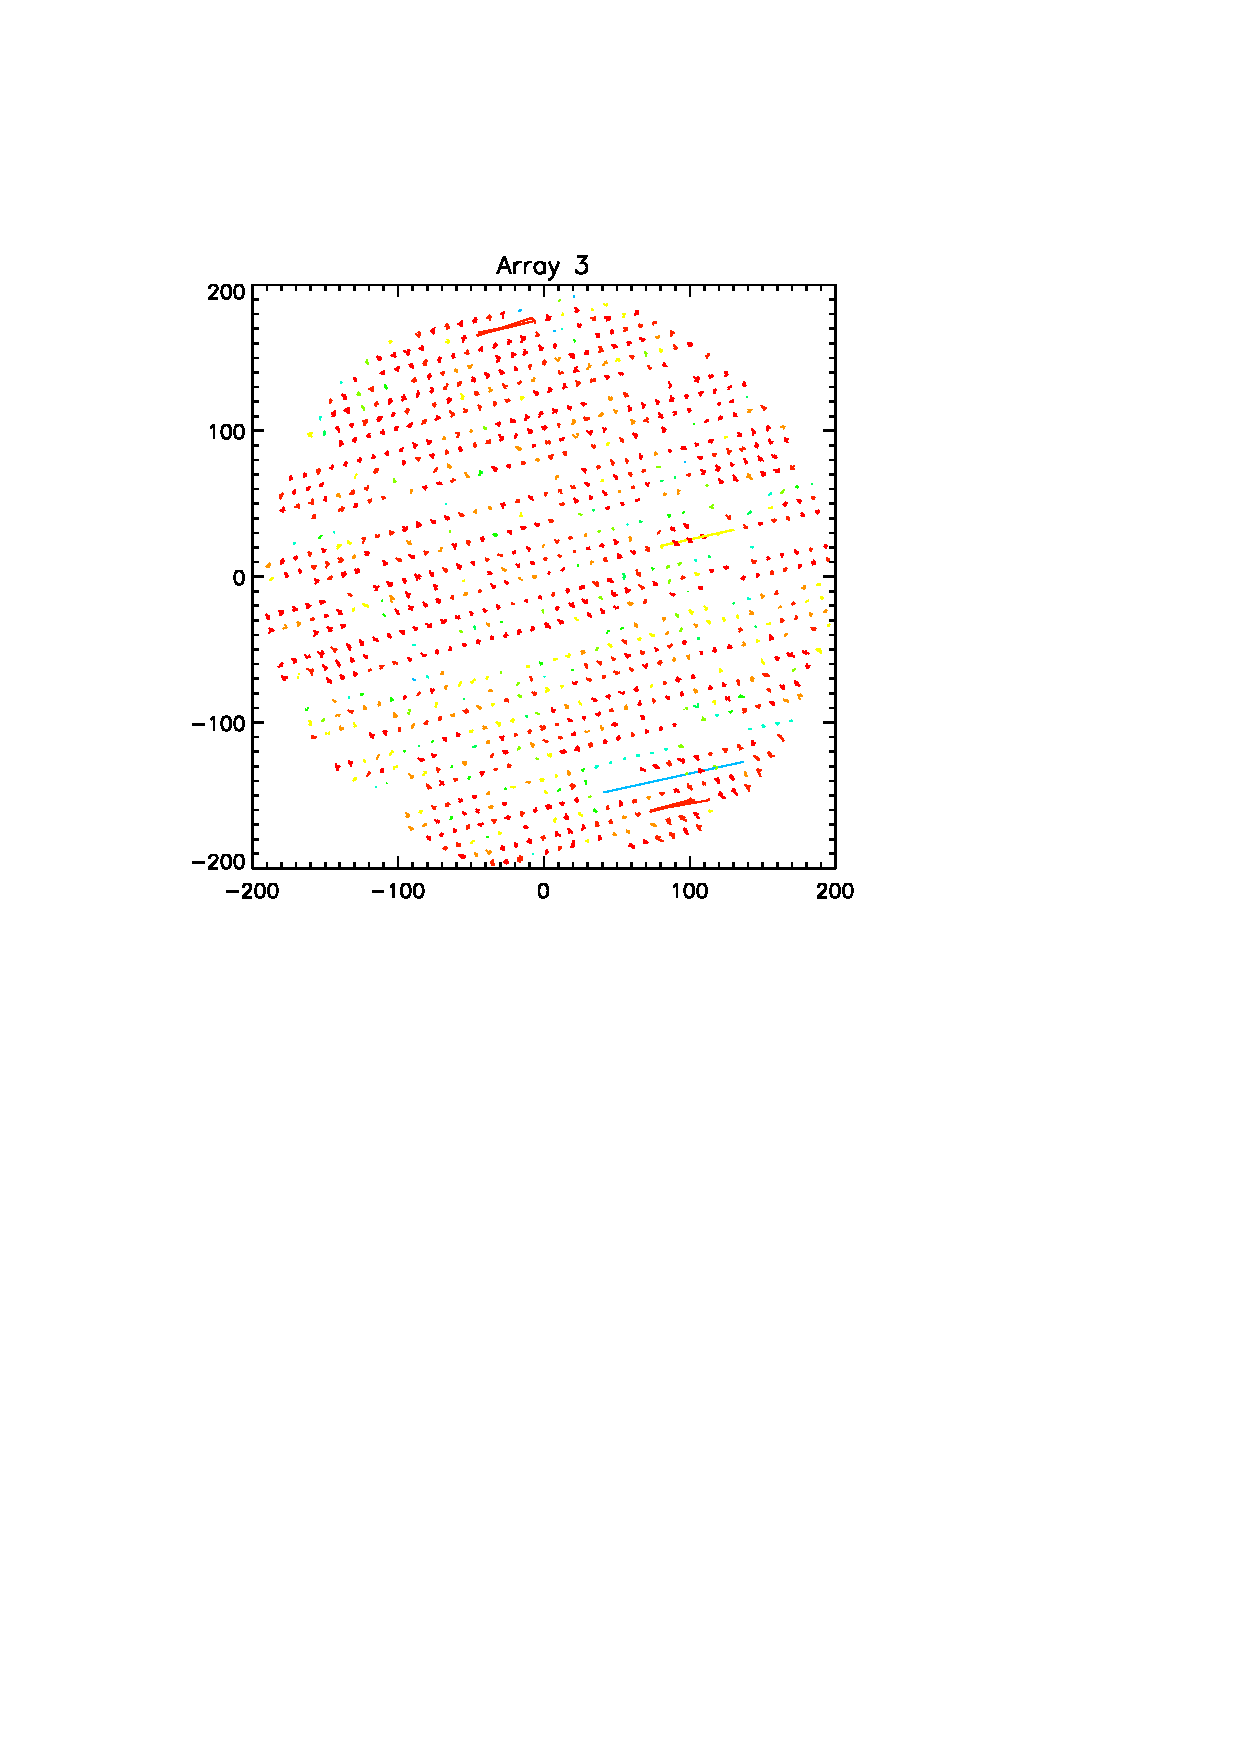
\includegraphics[trim=2cm 14cm 5cm 4cm, clip=true,width=0.55\linewidth]{Figures/A3_positions.pdf}
%% 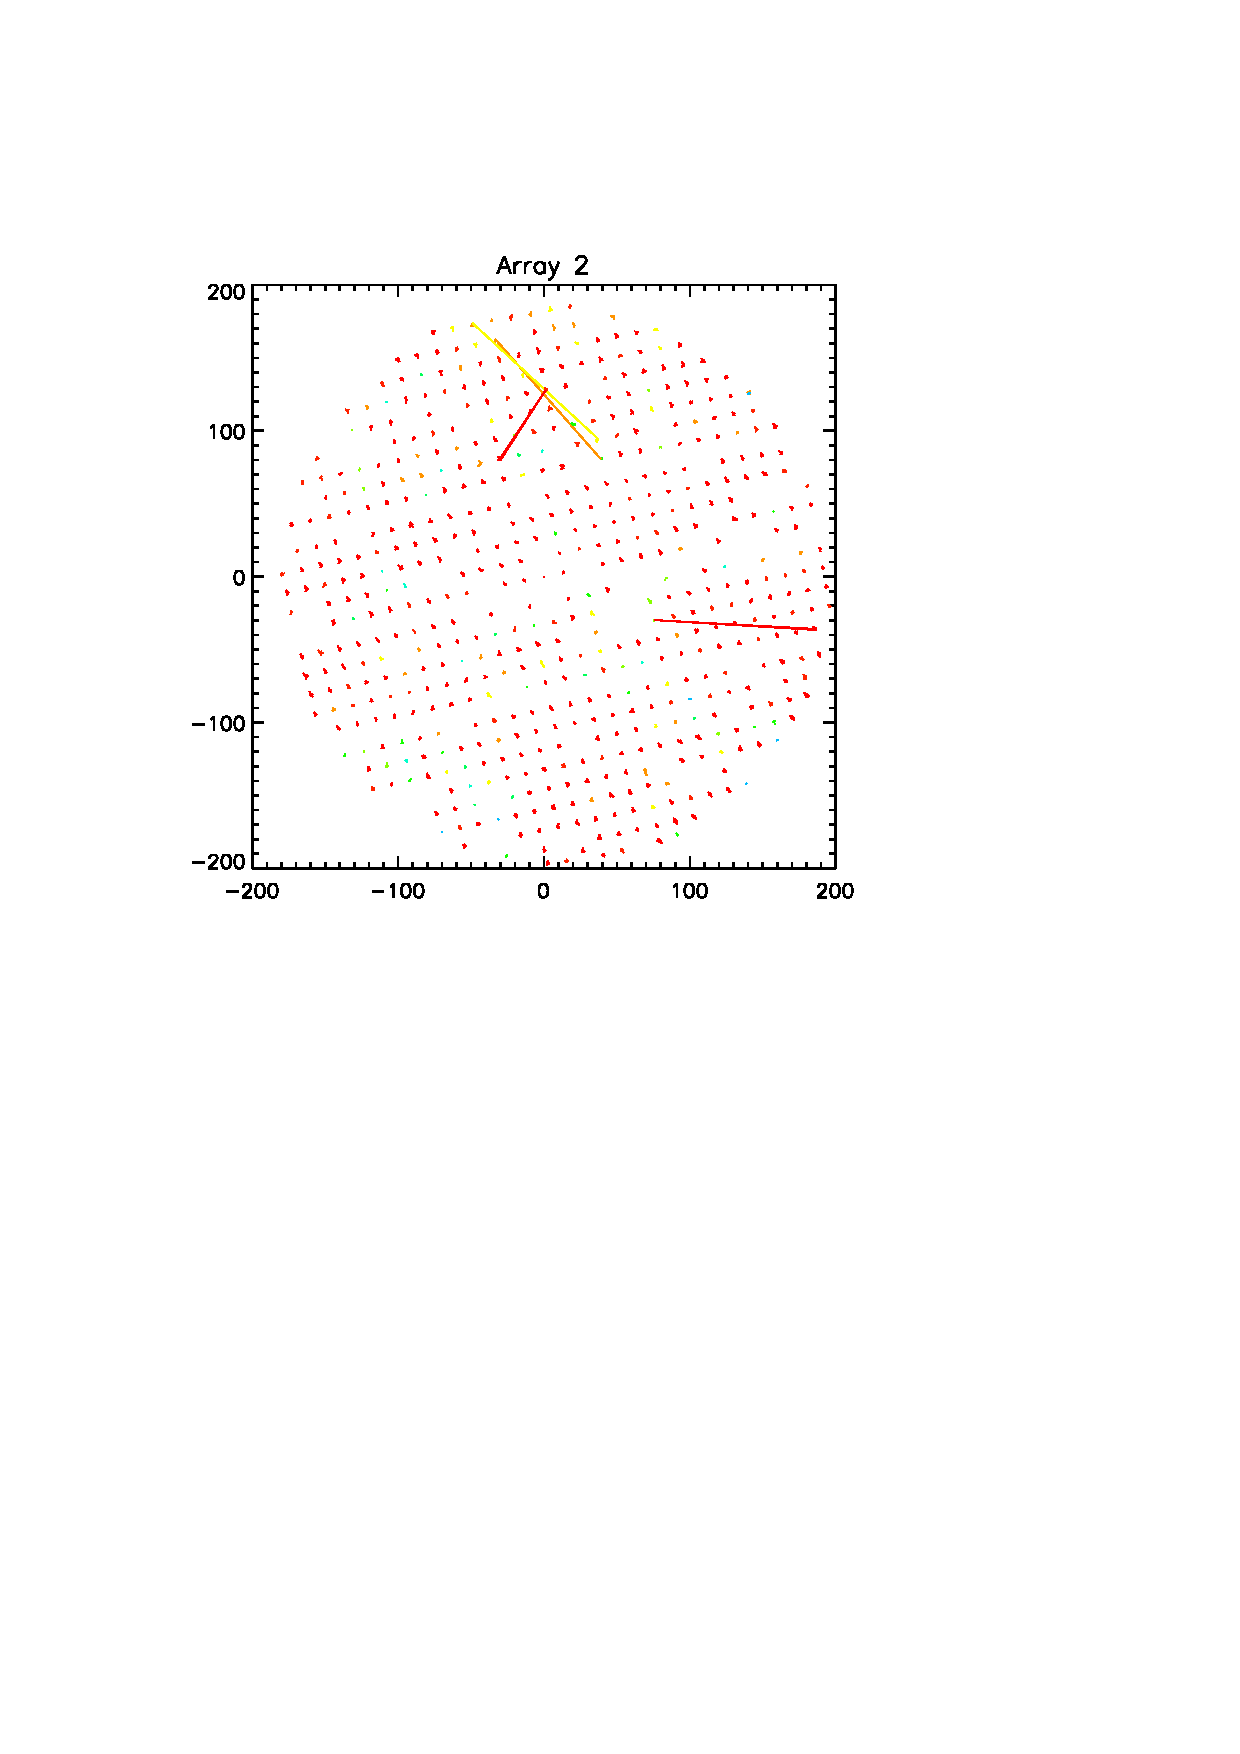
\includegraphics[trim=2cm 14cm 5cm 4cm, clip=true,width=0.55\linewidth]{Figures/A2_positions.pdf}
%% \caption[Stability of KID positions in the field-of-view]{For the valid
%%   detectors, we show the positions of each pixel, as obtained from each beam
%%   map. Some of them are not found at the same position for all the \bms.
%% Units are arcseconds. \todo{{\bf FM : color code : same as on the 1st
%%       maps of validity}}}
%% \label{fig:jumping_kids}
%% \end{center}
%% \end{figure}

%\begin{figure}[htp]
%\begin{center}
%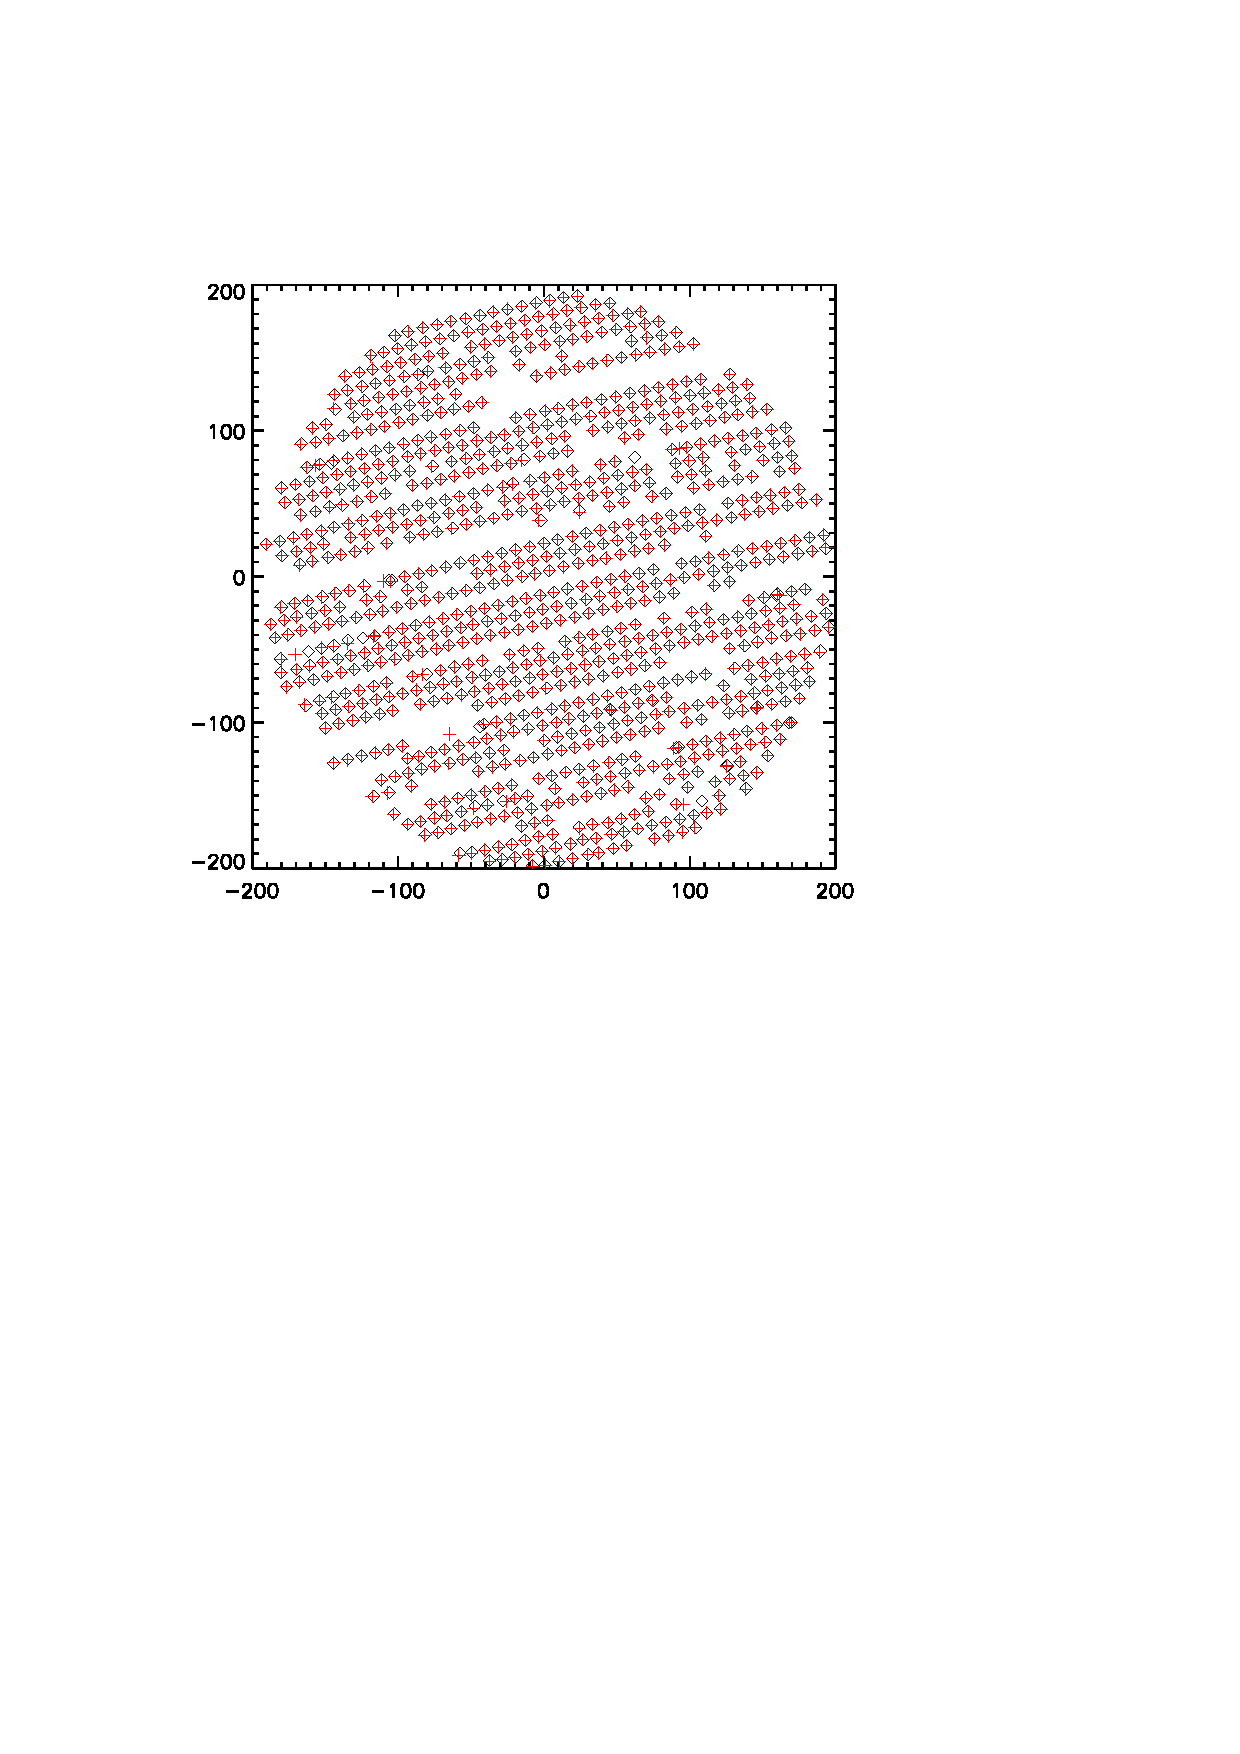
\includegraphics[trim=2cm 14cm 5cm 4cm, clip=true,width=0.55\linewidth]{Figures/A1_test_positions.pdf}
%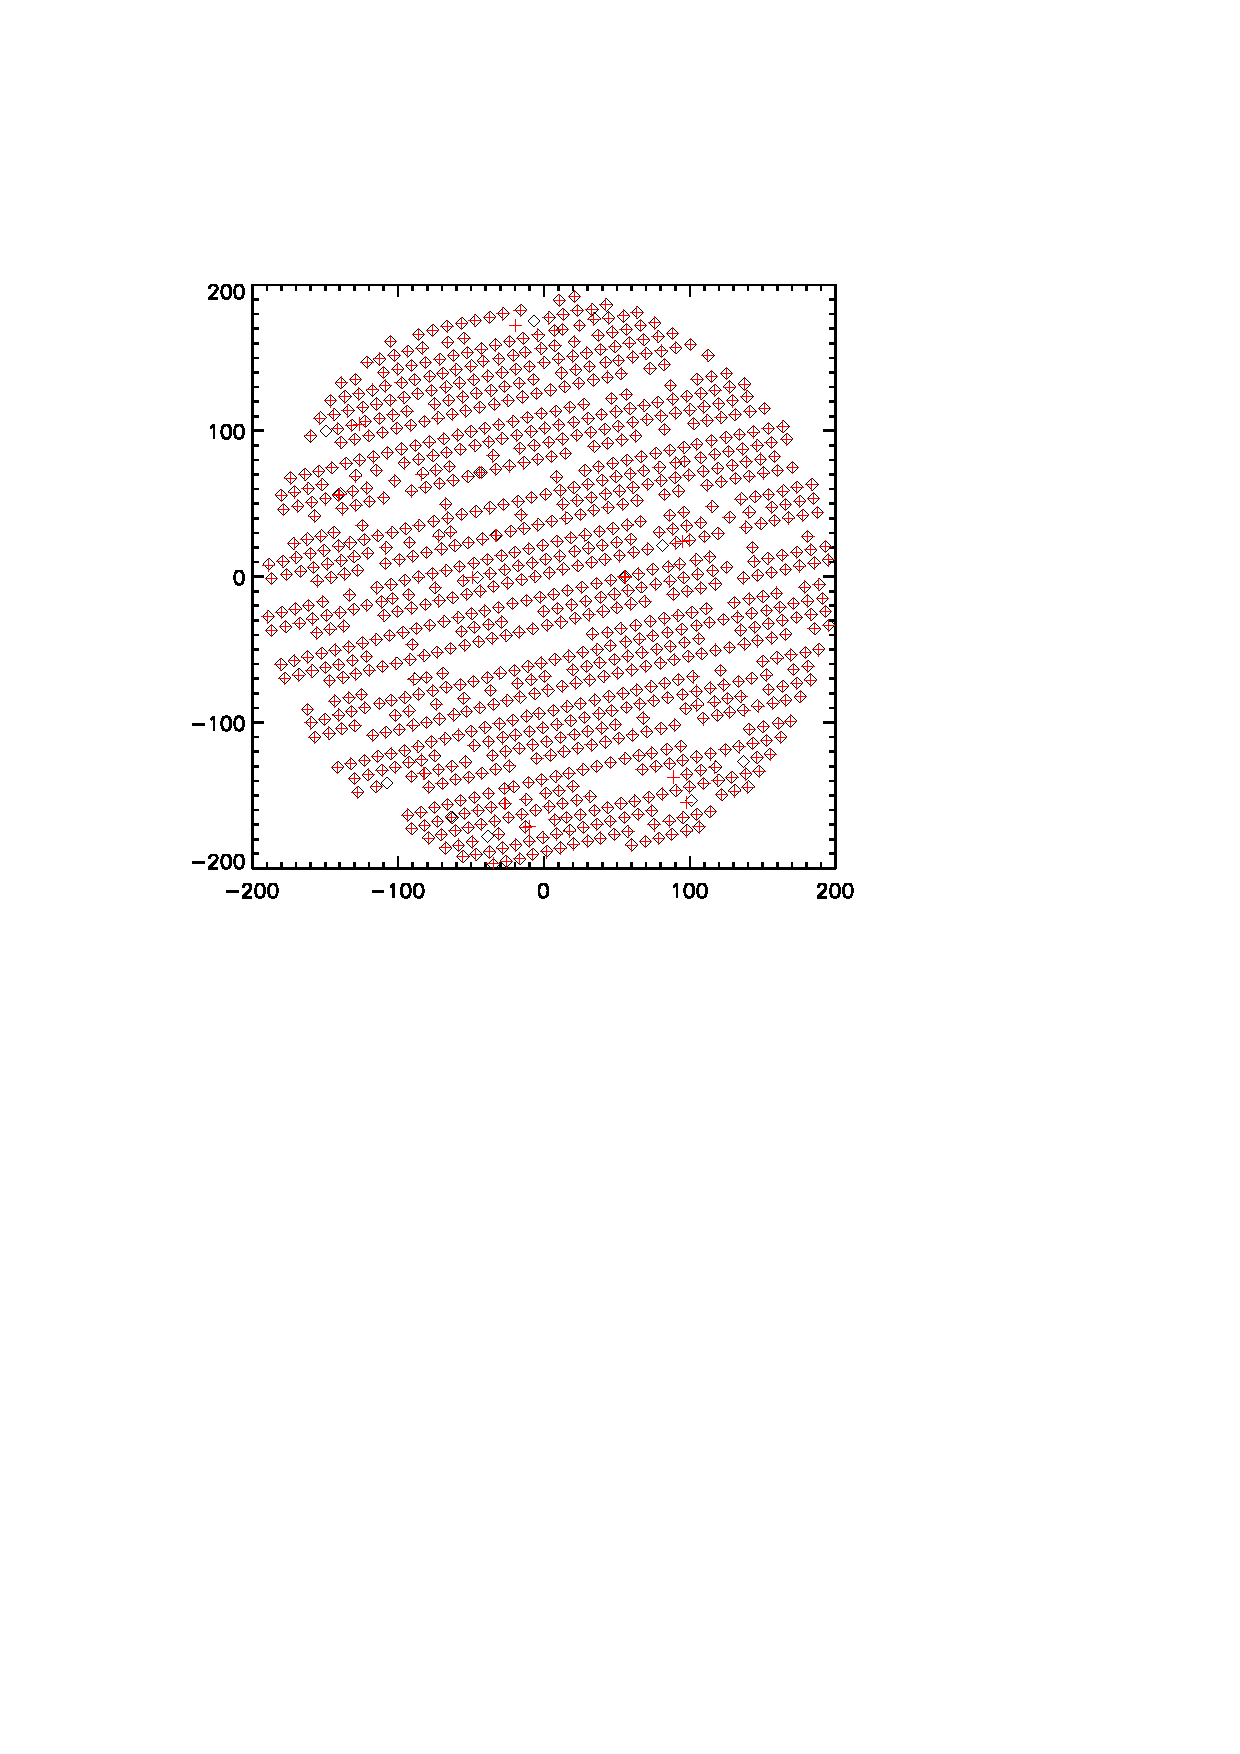
\includegraphics[trim=2cm 14cm 5cm 4cm, clip=true,width=0.55\linewidth]{Figures/A3_test_positions.pdf}
%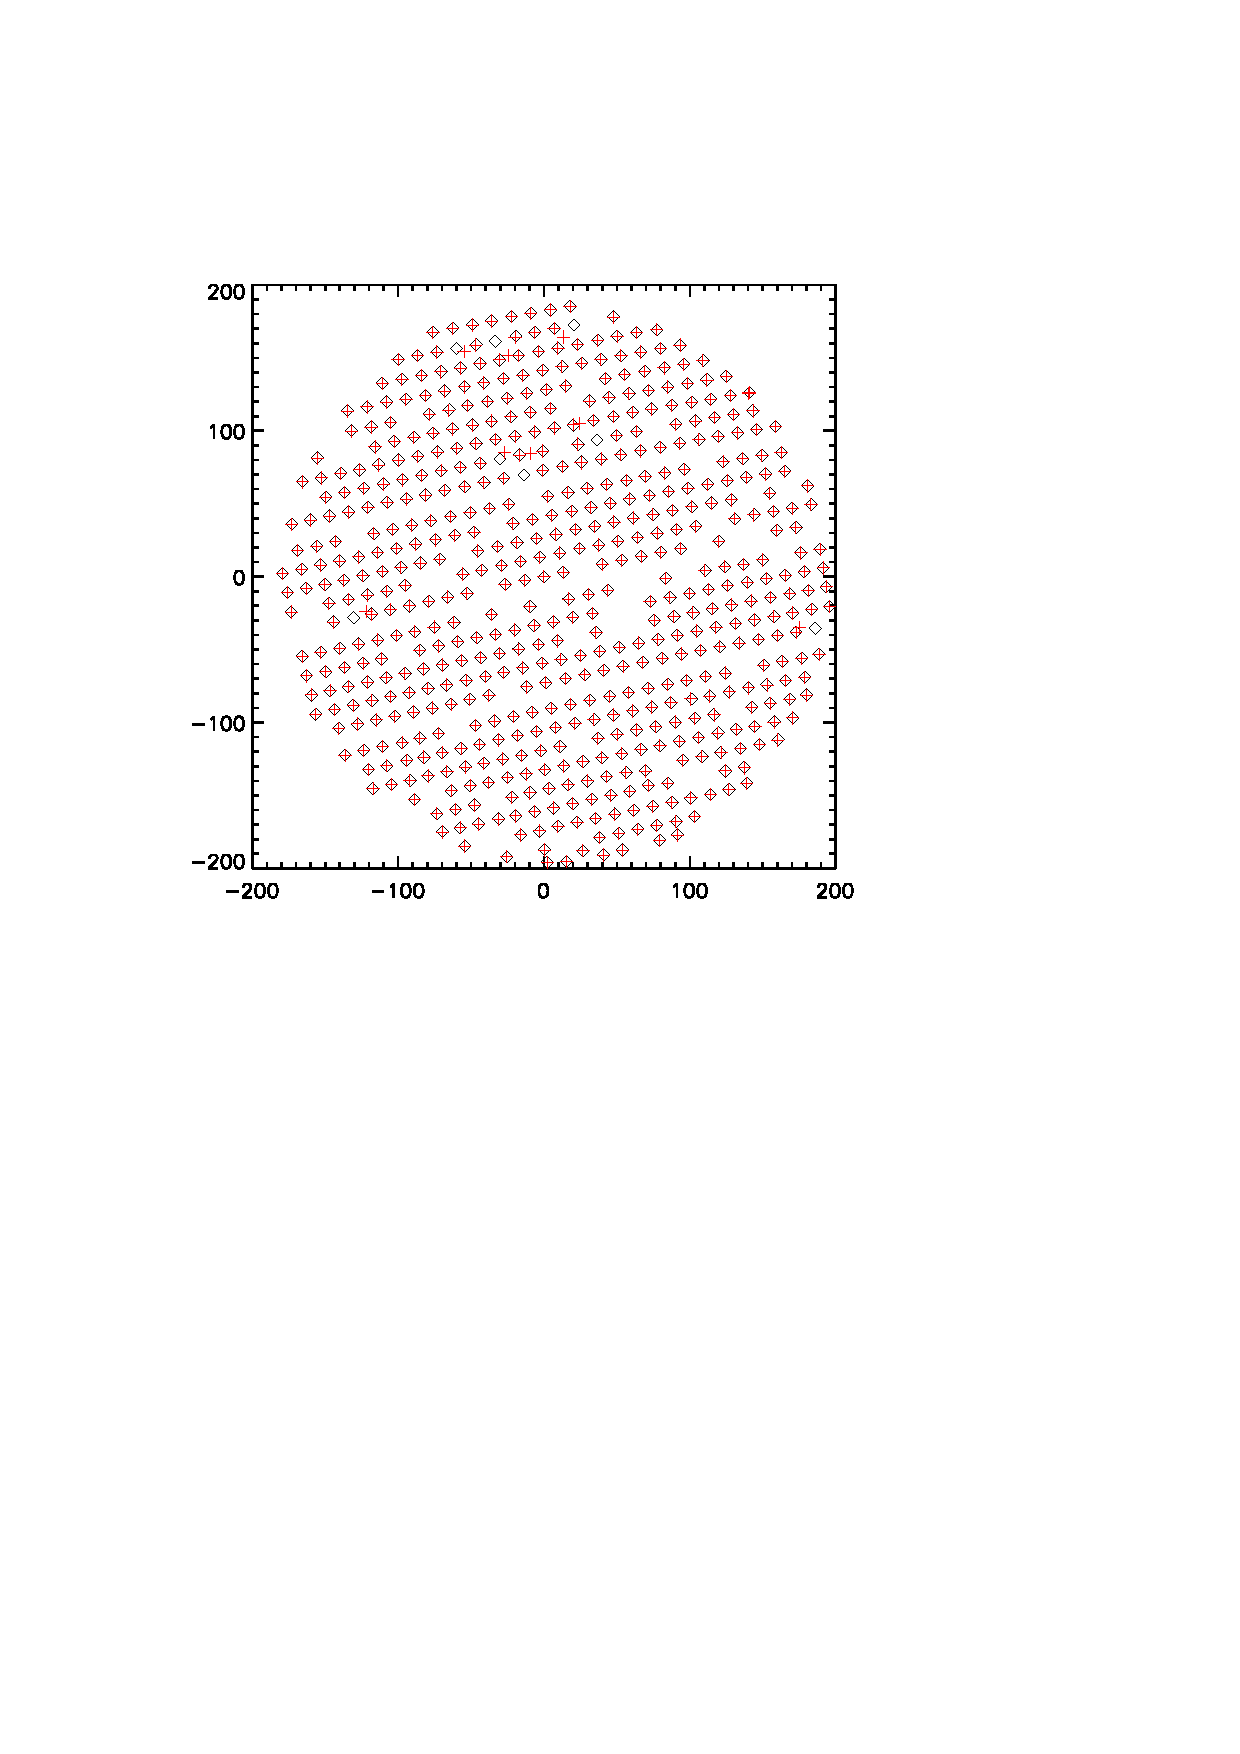
\includegraphics[trim=2cm 14cm 5cm 4cm, clip=true,width=0.55\linewidth]{Figures/A2_test_positions.pdf}
%\caption[Average KID positions]{For the valid detectors,
%  we show the mean (red crosses) and the median (black squares)
%  positions of each pixel, as obtained from each \bm.
%  Units are arcseconds. \todo{FM : color code ? same as on the 1st maps of validity}}
%\label{fig:mean_vs_median}
%\end{center}
%\end{figure}

\begin{table}[!htbp]
  \begin{center}
    \caption[Number of detectors]{Summary of the number of valid detectors per array.}
    \label{tab:number_of_kids}  
    \begin{tabular}{lrrr}
      \hline
      \hline
      \noalign{\smallskip}
      Characteristics & Array 1 & Array 3  & Array 2  \\
      \noalign{\smallskip}
      \hline
      \noalign{\smallskip}
      Designed detectors ($N_k$)  & 1140  & 1140   & 616  \\
      Valid detectors             & 952   & 961    & 553  \\ 
      Ratio $\equiv \eta$         & 0.84  & 0.84   & 0.90   \\
      \noalign{\smallskip}
      \hline
    \end{tabular}
  \end{center}    
\end{table}

